\documentclass{article}
\usepackage[utf8]{inputenc}
\usepackage[T1]{fontenc}
\usepackage{graphicx}
\usepackage{algorithm}
\usepackage{algpseudocode}

\usepackage{listings}
\usepackage{xcolor}
\usepackage[margin=2cm]{geometry}
\usepackage{float}

\usepackage{amssymb} %Ajoute des symboles mathématiques comme R, Z, forall, exists, etc....
\usepackage{amsmath}
\usepackage{amsthm}

\usepackage{enumitem}


\lstdefinestyle{monstyle}{
    backgroundcolor=\color{white},
    commentstyle=\color{gray},
    keywordstyle=\color{blue},
    numberstyle=\tiny\color{gray},
    basicstyle=\ttfamily\small,
    breaklines=true,
    numbers=left,
    numbersep=5pt,
    frame=single,
}
\lstset{style=monstyle}


\usepackage{soul} % IMPORTANT : POUR SURLIGNER AVEC \hl en fin de ligne 
\usepackage{xcolor}


\title{\sethlcolor{purple!30}\hl{\textbf{Fiche de révisions : Environnement de travail -- GitHub}}}
\author{Derrez Lorenzo}

\begin{document}
\maketitle

\section*{\hl{\textbf{Introduction}}}

\subsection*{\textbf{Situations courantes}}
\begin{itemize}
    \item développer plusieurs projets, seul ou à plusieurs; 
    \item travailler à plusieurs sur les mêmes fichiers; 
    \item oublier une modification, vouloir la retrouver ou l'annuler.
\end{itemize}

\subsection*{\textbf{Besoin}}

\begin{itemize}
    \item GitHub $ \implies $ garde l'historique des modifications
    \item \qquad  \qquad $ \implies $ permet de revenir en arrière 
    \item \qquad  \qquad $ \implies $ gérer les conflits lorsque plusieurs personnes modifient le même fichier.
\end{itemize}

\section*{\hl{\textbf{Fonctionnement de base de Git}}}

\textbf{Distingue plusieurs espaces. Comprendre où se trouve une modification permet de comprendre les commandes de bases.}

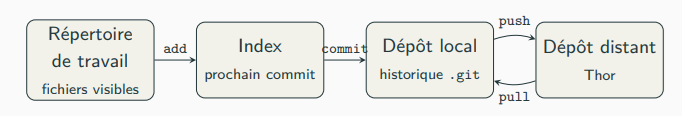
\includegraphics[width=0.50\textwidth]{fonctio_git.png}

\subsection*{\textbf{Cycle de travail avec Git}}

\begin{itemize}
    \item \sethlcolor{pink!30}\hl{git pull} : avant de commencer pour récupérer les modifications.
    \item \sethlcolor{pink!30}\hl{git status fichier} : permet de regarder la situations des fichiers (ajoutés, non ajoutés, etc..)
    \item \sethlcolor{pink!30}\hl{git diff fichier} : permet de regarder les différences entre deux fichiers.
    \item \sethlcolor{pink!30}\hl{git add fichier} : permet d'ajouter un fichier 
    \item \sethlcolor{pink!30}\hl{git commit -m "Message"} : permet de faire un commit sur le dépôt avec un message clair.
    \item \sethlcolor{pink!30}\hl{git push} : lorsque le commit est prêt on peut push sur le dépôt les modifications.
    \item \sethlcolor{pink!30}\hl{git clone repo} : première copie locale
\end{itemize}

\textbf{Remarque} : il est possible dans le fichier fichier /.gitconfig d'ajouter des données permettant d'améliorer la configuration du git.

\textbf{Remarque} : l'intérêt est d'utiliser une clé SSH pour relier Thor / GitHub pour faire un dépôt sécurisé.


\end{document}